\documentclass{standalone}

\usepackage{tikz}

\usetikzlibrary{positioning, chains, shapes.geometric, fit, shapes, arrows.meta, calc}

\begin{document}

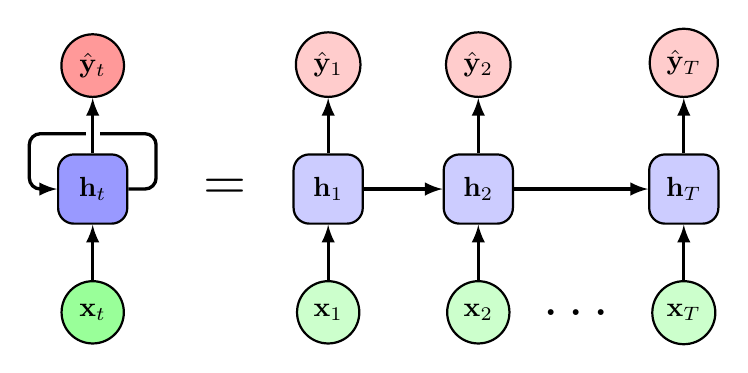
\begin{tikzpicture}[
    >=LaTeX, % Use default LaTeX arrows
    % Styles 
    cell/.style={ % RNN cell
        rectangle,
        rounded corners=2mm,
        minimum height=2.5em,
        minimum width=2.5em,
        draw,
        thick,
        fill=blue!40
    }, 
    cellc/.style={ % RNN cells in a chain
        cell,
        on chain,
        join,
        fill=blue!20
    },
    input/.style={ % Input or output node
        circle,
        minimum width=2.25em,
        draw,
        fill=green!20,
        thick
    },
    output/.style={ % Output node
        circle,
        minimum width=2.25em,
        draw,
        fill=red!20,
        thick
    },
    arrow/.style={
        -latex,
        very thick
    },
    arrowc1/.style={ % Arrows with rounded corners
        arrow,
        rounded corners=.25cm
    },
    arrowc2/.style={ % Arrows with big rounded corners
        arrow,
        rounded corners=.5cm
    }
]

    % RNN
    \begin{scope}[start chain=going right, nodes=cellc, arrow, local bounding box=chain]
        \path[shift={(-9em, 1em)}] 
            node (h1) {$\mathbf{h}_1$}
            node[] (h2) {$\mathbf{h}_2$}
            node[xshift=2em] (hT) {$\mathbf{h}_{T}$};
    \end{scope}

    % Inputs and arrows from inputs
    \foreach \X in {1, 2, T} {
        \draw[arrow, latex-] (h\X.south) -- ++ (0, -2em)
            node[below, input] (x\X) {$\mathbf{x}_\X$};
    }

    % Outputs and arrows to outputs
    \foreach \X in {1, 2, T} {
        \draw[arrow] (h\X.north) -- ++ (0, 2em)
            node[above, output] (y\X) {$\hat{\mathbf{y}}_\X$};
    }

    % Continuation dots
    \path (x2) -- (xT) node[midway, scale=2] {\dots};

    % Equals
    \node[left=1em of chain, scale=2] (eq) {$=$};

    % Unfolded RNN
    \node[cell, left=2em of eq] (AL) {$\mathbf{h}_t$};
    \path (AL.west) ++ (-1em,2em) coordinate (aux);
    \draw[arrow, rounded corners] (AL.east) -| ++ (1em, 2em) -- (aux) |- (AL.west);
    \draw[white, line width=0.5em] (AL.north) -- ++ (0, 1.9em);
    \draw[arrow] (AL.north) -- ++ (0, 2em)
        node[above,output,fill=red!40] {$\hat{\mathbf{y}}_t$};
    \draw[arrow, latex-] (AL.south) -- ++ (0, -2em)
        node[below,input,fill=green!40] {$\mathbf{x}_t$};
\end{tikzpicture}

\end{document}